\documentclass[tikz,border=6pt]{standalone}
\usepackage{pgfplots}
\pgfplotsset{compat=1.18}
\usetikzlibrary{positioning,arrows.meta}
\begin{document}
% Hardware-efficiency Pareto: FPS vs. Power.
% Labels placed INSIDE plot area to keep tight bounding box when scaled to column width.
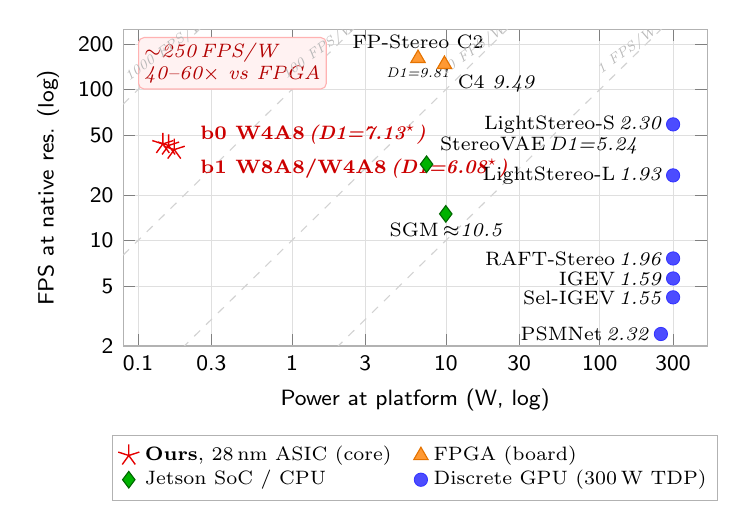
\begin{tikzpicture}
\begin{axis}[
  width=9cm, height=5.6cm,
  xmode=log, ymode=log,
  xlabel={Power at platform (W, log)},
  ylabel={FPS at native res. (log)},
  xmin=0.08, xmax=500,
  ymin=2.0, ymax=250,
  xtick={0.1,0.3,1,3,10,30,100,300},
  xticklabels={0.1, 0.3, 1, 3, 10, 30, 100, 300},
  ytick={2,5,10,20,50,100,200},
  yticklabels={2, 5, 10, 20, 50, 100, 200},
  grid=major, grid style={line width=0.2pt, gray!25},
  axis line style={gray!60},
  font=\sffamily\footnotesize,
  legend style={at={(0.5,-0.28)}, anchor=north,
                font=\scriptsize, draw=black!30, fill=white, inner sep=2pt,
                row sep=-2pt, legend columns=2,
                /tikz/every even column/.append style={column sep=6pt}},
  legend cell align=left,
  clip=true,
]
% --------- Energy-efficiency isolines (FPS = k * Power), clipped to plot ---------
\foreach \k in {1000, 100, 10, 1}{
  \addplot[domain=0.08:500, samples=2, gray!35, dashed, line width=0.4pt, forget plot]
    {\k * x};
}

% --------- Ours (red stars) ---------
\addplot+[only marks, mark=star, mark size=4pt,
          mark options={fill=red!70, draw=red!90!black, line width=0.5pt}]
  coordinates {(0.145,43.6) (0.158,42.6) (0.172,40.0)};
\addlegendentry{\textbf{Ours}, 28\,nm ASIC (core)}

% --------- FPGA (orange triangles) ---------
\addplot+[only marks, mark=triangle*, mark size=3pt,
          mark options={fill=orange!80, draw=orange!90!black, line width=0.4pt}]
  coordinates {(6.6,161) (9.8,147)};
\addlegendentry{FPGA (board)}

% --------- Embedded SoC/CPU (green diamonds) ---------
\addplot+[only marks, mark=diamond*, mark size=3pt,
          mark options={fill=green!70!black, draw=green!40!black, line width=0.4pt}]
  coordinates {(7.5,32) (10,15)};
\addlegendentry{Jetson SoC / CPU}

% --------- Discrete GPU (blue circles) ---------
\addplot+[only marks, mark=*, mark size=2.4pt,
          mark options={fill=blue!70, draw=blue!80, line width=0.3pt}]
  coordinates {(300,58.8) (300,27.0) (300,7.6) (300,5.6) (300,4.2) (250,2.4)};
\addlegendentry{Discrete GPU (300\,W TDP)}

% ========== LABELS — all anchored INSIDE plot to keep bounding box tight ==========

% Ours: two lines to the right of star cluster
\node[font=\scriptsize\bfseries, red!80!black, anchor=west]
  at (axis cs:0.22,50)   {b0 W4A8\,\scriptsize\itshape(D1=7.13$^\star$)};
\node[font=\scriptsize\bfseries, red!80!black, anchor=west]
  at (axis cs:0.22,30)   {b1 W8A8/W4A8\,\scriptsize\itshape(D1=6.08$^\star$)};

% Callout near our stars
\node[font=\scriptsize\itshape, red!70!black, anchor=south west, align=left,
      fill=red!5, draw=red!30, rounded corners=2pt, inner sep=2pt]
  at (axis cs:0.10,100) {$\sim$250\,FPS/W\\40--60$\times$ vs FPGA};

% FPGA
\node[font=\scriptsize, anchor=south]      at (axis cs:6.6,161)  {FP-Stereo C2};
\node[font=\tiny\itshape, anchor=north]    at (axis cs:6.6,161)  {D1=9.81};
\node[font=\scriptsize, anchor=north west] at (axis cs:9.8,145)  {\,C4 \itshape 9.49};

% SoC/CPU
\node[font=\scriptsize, anchor=south west] at (axis cs:7.5,32)   {\,StereoVAE\,\itshape D1=5.24};
\node[font=\scriptsize, anchor=north]      at (axis cs:10,15)    {SGM\,\itshape$\approx$10.5};

% GPU (anchor=east, labels go LEFT of markers to stay inside plot)
\node[font=\scriptsize, anchor=east] at (axis cs:290,58.8) {LightStereo-S\,\itshape 2.30};
\node[font=\scriptsize, anchor=east] at (axis cs:290,27.0) {LightStereo-L\,\itshape 1.93};
\node[font=\scriptsize, anchor=east] at (axis cs:290,7.6)  {RAFT-Stereo\,\itshape 1.96};
\node[font=\scriptsize, anchor=east] at (axis cs:290,5.6)  {IGEV\,\itshape 1.59};
\node[font=\scriptsize, anchor=east] at (axis cs:290,4.2)  {Sel-IGEV\,\itshape 1.55};
\node[font=\scriptsize, anchor=east] at (axis cs:240,2.4)  {PSMNet\,\itshape 2.32};

% Isoline labels, placed INSIDE plot at upper portion
\node[font=\tiny\itshape, gray!55, rotate=36] at (axis cs:0.15,180) {1000 FPS/W};
\node[font=\tiny\itshape, gray!55, rotate=36] at (axis cs:1.5,180)  {100 FPS/W};
\node[font=\tiny\itshape, gray!55, rotate=36] at (axis cs:15,180)   {10 FPS/W};
\node[font=\tiny\itshape, gray!55, rotate=36] at (axis cs:150,180)  {1 FPS/W};

\end{axis}
\end{tikzpicture}
\end{document}
